\documentclass[../../main.tex]{subfiles}

\graphicspath{{\subfix{../../immagini/}}}

\begin{document}
    Un possibile miglioramento della struttura dell'LBF descritta nel paragrafo precedente viene fornita dal \textit{sandwiched learned Bloom filter}, nel quale l'efficienza dell'LBF viene aumentata aggiungendo un nuovo filtro di Bloom che precede il modello.

    In questa nuova tipologia di filtro il processo di verifica dell'appartenenza all'insieme delle chiavi avviene quindi in questo modo: un elemento $x$ viene passato in ingresso al filtro, se questo etichetta l'elemento come non-chiave allora $x$ non è una chiave (essendo un filtro classico non possono essere presenti falsi negativi); viceversa, se $x$ viene giudicato come appartenente all'insieme delle chiavi allora viene passato in ingresso al modello, da qui in poi il processo è equivalente a quello di un LBF.

    Intuitivamente l'efficienza di questa struttura è superiore rispetto ad un LBF perché il filtro iniziale fornisce subito una `scrematura' degli elementi delle query. Questo permette di diminuire il numero di falsi positivi generati dal classificatore e, di conseguenza, avere un filtro di backup con una dimensione inferiore rispetto alla controparte dell'LBF.

    Grazie al filtro iniziale, un SLBF risulta inoltre più robusto rispetto ad un LBF: come spiegato nel paragrafo precedente infatti il tasso di falsi positivi in un LBF può variare molto a seconda delle query che gli vengono presentate, questo problema in un SLBF viene mitigato perché, supponendo di avere una query $\mathcal{Q}$, il classificatore dell'SLBF dovrà lavorare su un numero minore di elementi (in quanto alcuni saranno già stati eliminati dal filtro iniziale) rispetto ad un LBF a cui viene presentata la stessa query.

    Formalmente, un SLBF può quindi essere definito come segue \cite{ma2020}: 

    ``Un SLBF $(B_0, g, \tau, B)$, definito su un insieme di chiavi $\mathcal{K}$ e un insieme di non-chiavi $\mathcal{U}$, è un LBF a cui viene aggiunto un ulteriore filtro di Bloom $B_0$, che prende il nome di filtro iniziale; questo filtro conterrà tutti gli elementi dell'insieme $\mathcal{K}$. Dato un qualsiasi elemento $x$, se il filtro iniziale restituisce $x \notin \mathcal{K}$,l'SLBF restituirà lo stesso risultato; viceversa, se il filtro iniziale ritorna $x \in \mathcal{K}$, il risultato dipenderà dall'LBF $(g, \tau, B)$ rimanente.''

    La Figura \ref{fig:DifferenzeFiltri} riassume il processo di verifica dell'appartenenza all'insieme delle chiavi di un generico elemento $x$ per le tre tipologie di filtro presentate.
    
    \begin{figure}[H]
        \centering
        \begin{subfigure}[c]{0.3\textwidth}
            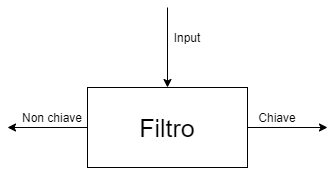
\includegraphics[width=\textwidth]{immagini/5_2/bloomFilter.png}
            \caption{}
            \label{fig:appartenenzaBF}
        \end{subfigure}
        \begin{subfigure}[c]{0.3\textwidth}
            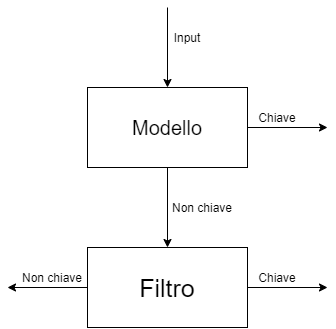
\includegraphics[width=\textwidth]{immagini/5_2/LBF.png}
            \caption{}
            \label{fig:appartenenzaLBF}
        \end{subfigure}
        \begin{subfigure}[c]{0.3\textwidth}
            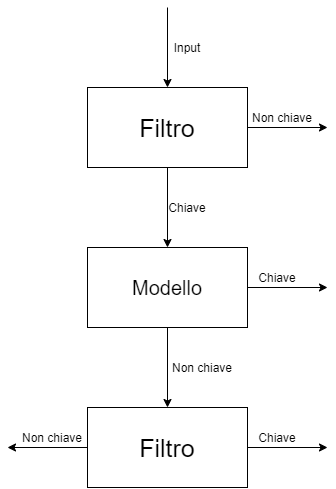
\includegraphics[width=\textwidth]{immagini/5_2/SLBF.png}
            \caption{}
            \label{fig:appartenenzaSLBF}
        \end{subfigure}
        \caption{Processo di verifica dell'appartenenza per le tre diverse tipologie di filtro: (a) nel caso di un filtro di Bloom, (b) nel caso di un LBF, (c) nel caso di un SLBF.}
        \label{fig:DifferenzeFiltri}
    \end{figure}
\end{document}